\chapter{Background}
\label{cha:bg}

This chapter will cover some of the background material required for the following sections, it will cover the history of reinforcement learning (RL) and it's evolution to the current state-of-the-art. Additionally, it will cover the related work to this project and also cover some details of the past research papers for which this project has been based upon.

\section{Reinforcement learning}
\label{bg:sec:rl}
Reinforcement learning is an area of machine learning has has been under active research since the late 1980s (TODO: ref watkins phd). The first defining algorithm of RL was called \textit{`temporal-difference learning'} often referred to as TD-Learning. This algorithm learns by bootstrapping from the current value function in order iteratively converge towards a optimal policy (i.e. the agent's strategy for taking actions in the environment).

Further work by R. Sutton led to the development of TD-Lambda, an algorithm that was applied to the game of Backgammon, in 1992, by Gerald Tesauro to create TD-Gammon(TODO: ref Tesauri paper). It was a computer program that was shown to compete at expert-human level. The program also found novel strategies that were either unexplored, or dismissed in error as poor strategies. This was the first example of RL aiding in discovery or reconsideration of board game strategies. This trend of RL algorithms helping to improve human play would prove to only continue with DeepMind's AlphaZero program mastering the games of Chess (beating the strongest Chess programs such as Stockfish\footnote{\href{https://stockfishchess.org}{Stockfish}. One of the strongest Chess programs based on the CCRL ratings list.}) and Go.

\subsection{Deep reinforcement learning}
\label{bg:sec:deeprl}
Following from section \ref{bg:sec:rl} on RL, this section talks about the combination of two areas, deep learning and reinforcement learning methods, called deep reinforcement learning (DRL). Deep learning (DL) is a common class of machine learning methods that has been of much research focus over the past decade and can deal with high-dimensional sensory input; for the case of Atari this is 84x84 greyscale images after pre-processing of the raw Atari frames. On the other hand, reinforcement learning allows us to create an agent which can learn an optimal policy to navigate some environment in order to optimise its reward.

\begin{figure}[htbp]
	\centering
	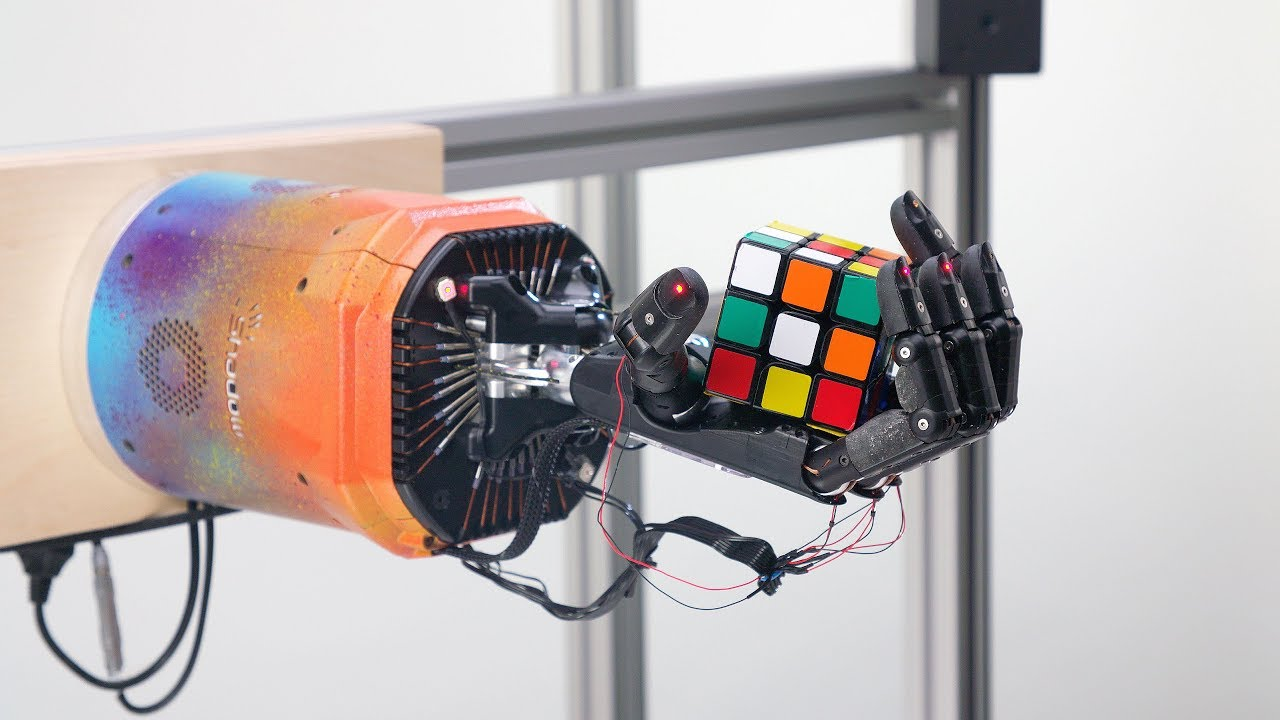
\includegraphics[width=0.5\textwidth]{chapters/chapter2/images/openai-robot.jpg}
	\caption{OpenAI Robot solving a Rubik's cube
		\label{fig:openai-robot}
	}
\end{figure}

Through the combination of these methods, it has proven to provide solutions to previously intractable problems \cite{rl-survey} in areas such as robotics, computer vision and healthcare. For example, in 2019 OpenAI developed a robotic hand that could solve a Rubik's cube \ref{fig:openai-robot}, trained using deep reinforcement learning. As an extension to DRL, end-to-end reinforcement learning is a method for single layered neural network, trained by reinforcement learning. Figure \ref{fig:e2e-rl} shows, diagramatically, how DL and RL are used together in order to produce a single end-to-end model. In this simple architcture, there are two main components, the agent and the environment. This is a key feature of all DRL methods, an agent observes some state and reward from the environment after taking an action.

\begin{figure}[htbp]
	\centering
	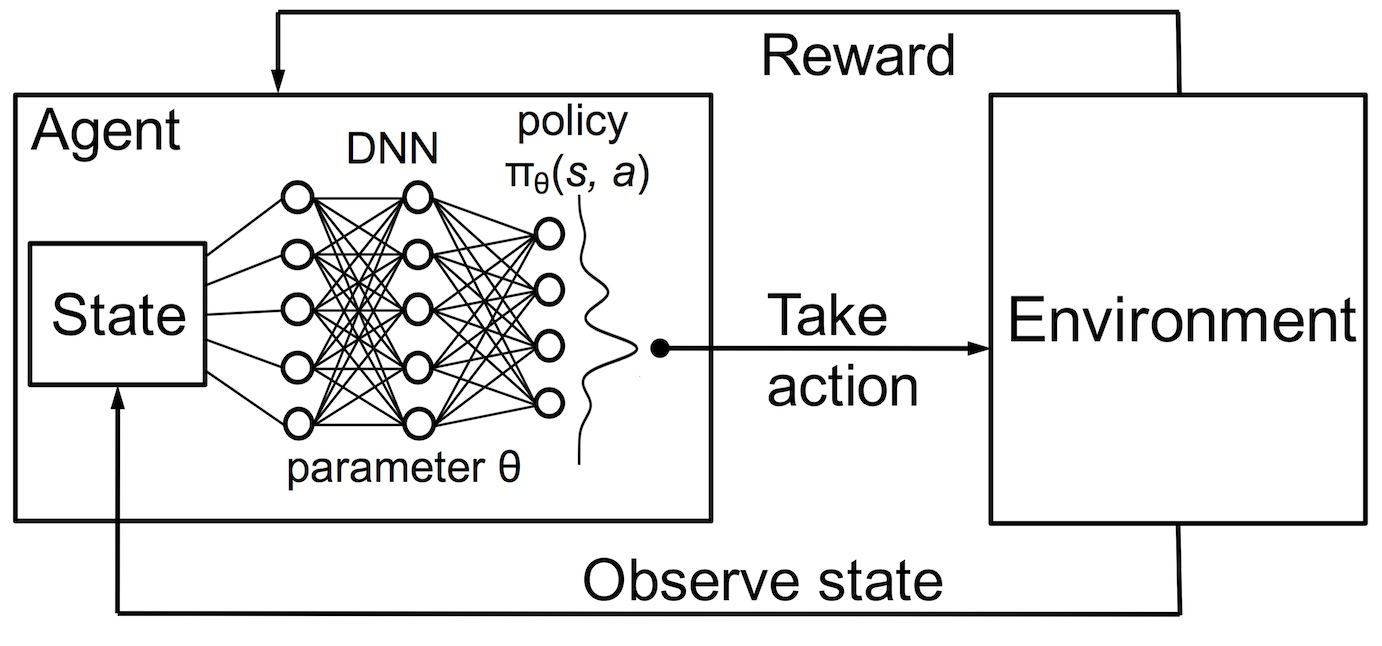
\includegraphics[width=0.5\textwidth]{chapters/chapter2/images/e2e-rl.jpg}
	\caption{Representation of end-to-end RL architctures
		\label{fig:e2e-rl}
	}
\end{figure}

Following on from Section \ref{bg:sec:rl}

\section{DQN on Atari 2600}
\label{bg:sec:dqn}
sdgsdsdfg

\section{CNN Visualisation}
\label{bg:sec:cnn-vis}
sdfsdfsdfsdfsdf